%% BACKGROUND (Wiktor) %%% 

\subsection {Real Time Computing}
%
Real-time computing is the study of hardware and software systems that must satisfy explicit 
response-time constraints or risk severe consequences, including failure. Timed systems are 
used in a wide range of domains including communications, embedded systems, real-time and automated control. 
They can be easily found in our environment; one of simple examples is the airbag system in a car. 
The real-time constraint in this system is the reaction time between crash sensors receiving input and 
the deployment of airbags. Among some of the important characteristics of real-time systems we can distinguish 
extreme reliability and safety as they are very often safety-critical.    

\subsection{ECDAR \label{background-ecdar}}
%
“Environment for Compositional Design and Analysis of Real Time Systems” - is a graphical tool based on UPPAAL TIGA[] that 
allows to visually create models of real-time systems. Unlike UPPAAL, it is implementing a complete specification theory for 
real time systems[]. In ECDAR[], components of the system are described as automatons extended with clocks (timed automata), 
that can be combined to form larger comprehensive system descriptions. Correct specification of composition is supported by 
well defined compositional reasoning theory, consisting of operators like: parallel composition, conjunction, satisfaction 
checking and refinement. On the top of that, the tool allows for scalable verification of models by querying the 
implementation with verification questions. 
%

\subsection{Timed Input/Output Automata \label{background-tioa}}
%
TI/OA is a basic, mathematical specification framework for description and analysis of real-time systems. 
In this framework, system is represented by nondeterministic, possibly infinite-state, state machine referred 
as “timed I/O automaton” (TIOA)[1]. TIOA has been implemented as specification formalism in a complete 
specification framework for real time systems.

\begin{figure}
\begin{centering}
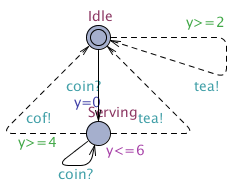
\includegraphics[scale=0.7]{images/bev_machine_model}
\par\end{centering}

\caption{Model of beverage serving machine.}
\end{figure}

In the preceding example, the TIOA consists of and two locations represented by 
circles: \emph{Idle} and \emph{Serving}, where \emph{Idle} represents the starting location and clock \emph{y} 
is defined. The flow of TIOA is controlled by three types of labels: \emph{guards}, \emph{invariants} and \emph{clock reset-operations}. 
Guards are located on the edges ($y>=2$ and $y>=4$) and express conditions on the values of clock that must be satisfied in order for 
the edge to be taken. Invariants are defined on locations ($y<=6$) and represent constraints for the clocks in order for the control to 
remain in particular location. Clock-reset operations ($y=0$) are simple clock value manipulations in form of assignment that enforce progress in the system.

%% //TO DO: Explain sync ! , ?

In ECDAR, the specification interface is leveraging the UPPAAL TIGA language[4] to describe TIOA. However, the following constraints are retained[]:   
%
\begin{itemize}
\item Invariants may not be strict.
\item Inputs must use controllable edges.
\item Outputs must use uncontrollable edges.
\item All channels must be declared broadcast.
\item The system is implicitly input enabled due to broadcast communication but for refinement checking purposes the relevant inputs must be explicit in the model.
\item In the case of parallel composition of several components, a given output must be exclusive to one component.
\item For implementations, outputs must be urgent.
\item For implementations, every state must have independent time progress, i.e., progress must be ensured by either an output or infinite delay.
\item Tau transitions (no output or input) are forbidden.
\item Global variables are forbidden.
\end{itemize}

\subsection{Anything else?}
%
...
%
